\documentclass[1p]{elsarticle_modified}
%\bibliographystyle{elsarticle-num}

%\usepackage[colorlinks]{hyperref}
%\usepackage{abbrmath_seonhwa} %\Abb, \Ascr, \Acal ,\Abf, \Afrak
\usepackage{amsfonts}
\usepackage{amssymb}
\usepackage{amsmath}
\usepackage{amsthm}
\usepackage{scalefnt}
\usepackage{amsbsy}
\usepackage{kotex}
\usepackage{caption}
\usepackage{subfig}
\usepackage{color}
\usepackage{graphicx}
\usepackage{xcolor} %% white, black, red, green, blue, cyan, magenta, yellow
\usepackage{float}
\usepackage{setspace}
\usepackage{hyperref}

\usepackage{tikz}
\usetikzlibrary{arrows}

\usepackage{multirow}
\usepackage{array} % fixed length table
\usepackage{hhline}

%%%%%%%%%%%%%%%%%%%%%
\makeatletter
\renewcommand*\env@matrix[1][\arraystretch]{%
	\edef\arraystretch{#1}%
	\hskip -\arraycolsep
	\let\@ifnextchar\new@ifnextchar
	\array{*\c@MaxMatrixCols c}}
\makeatother %https://tex.stackexchange.com/questions/14071/how-can-i-increase-the-line-spacing-in-a-matrix
%%%%%%%%%%%%%%%

\usepackage[normalem]{ulem}

\newcommand{\msout}[1]{\ifmmode\text{\sout{\ensuremath{#1}}}\else\sout{#1}\fi}
%SOURCE: \msout is \stkout macro in https://tex.stackexchange.com/questions/20609/strikeout-in-math-mode

\newcommand{\cancel}[1]{
	\ifmmode
	{\color{red}\msout{#1}}
	\else
	{\color{red}\sout{#1}}
	\fi
}

\newcommand{\add}[1]{
	{\color{blue}\uwave{#1}}
}

\newcommand{\replace}[2]{
	\ifmmode
	{\color{red}\msout{#1}}{\color{blue}\uwave{#2}}
	\else
	{\color{red}\sout{#1}}{\color{blue}\uwave{#2}}
	\fi
}

\newcommand{\Sol}{\mathcal{S}} %segment
\newcommand{\D}{D} %diagram
\newcommand{\A}{\mathcal{A}} %arc


%%%%%%%%%%%%%%%%%%%%%%%%%%%%%5 test

\def\sl{\operatorname{\textup{SL}}(2,\Cbb)}
\def\psl{\operatorname{\textup{PSL}}(2,\Cbb)}
\def\quan{\mkern 1mu \triangleright \mkern 1mu}

\theoremstyle{definition}
\newtheorem{thm}{Theorem}[section]
\newtheorem{prop}[thm]{Proposition}
\newtheorem{lem}[thm]{Lemma}
\newtheorem{ques}[thm]{Question}
\newtheorem{cor}[thm]{Corollary}
\newtheorem{defn}[thm]{Definition}
\newtheorem{exam}[thm]{Example}
\newtheorem{rmk}[thm]{Remark}
\newtheorem{alg}[thm]{Algorithm}

\newcommand{\I}{\sqrt{-1}}
\begin{document}

%\begin{frontmatter}
%
%\title{Boundary parabolic representations of knots up to 8 crossings}
%
%%% Group authors per affiliation:
%\author{Yunhi Cho} 
%\address{Department of Mathematics, University of Seoul, Seoul, Korea}
%\ead{yhcho@uos.ac.kr}
%
%
%\author{Seonhwa Kim} %\fnref{s_kim}}
%\address{Center for Geometry and Physics, Institute for Basic Science, Pohang, 37673, Korea}
%\ead{ryeona17@ibs.re.kr}
%
%\author{Hyuk Kim}
%\address{Department of Mathematical Sciences, Seoul National University, Seoul 08826, Korea}
%\ead{hyukkim@snu.ac.kr}
%
%\author{Seokbeom Yoon}
%\address{Department of Mathematical Sciences, Seoul National University, Seoul, 08826,  Korea}
%\ead{sbyoon15@snu.ac.kr}
%
%\begin{abstract}
%We find all boundary parabolic representation of knots up to 8 crossings.
%
%\end{abstract}
%\begin{keyword}
%    \MSC[2010] 57M25 
%\end{keyword}
%
%\end{frontmatter}

%\linenumbers
%\tableofcontents
%
\newcommand\colored[1]{\textcolor{white}{\rule[-0.35ex]{0.8em}{1.4ex}}\kern-0.8em\color{red} #1}%
%\newcommand\colored[1]{\textcolor{white}{ #1}\kern-2.17ex	\textcolor{white}{ #1}\kern-1.81ex	\textcolor{white}{ #1}\kern-2.15ex\color{red}#1	}

{\Large $\underline{12a_{0451}~(K12a_{0451})}$}

\setlength{\tabcolsep}{10pt}
\renewcommand{\arraystretch}{1.6}
\vspace{1cm}\begin{tabular}{m{100pt}>{\centering\arraybackslash}m{274pt}}
\multirow{5}{120pt}{
	\centering
	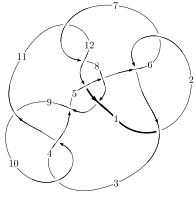
\includegraphics[width=112pt]{../../../GIT/diagram.site/Diagrams/png/1252_12a_0451.png}\\
\ \ \ A knot diagram\footnotemark}&
\allowdisplaybreaks
\textbf{Linearized knot diagam} \\
\cline{2-2}
 &
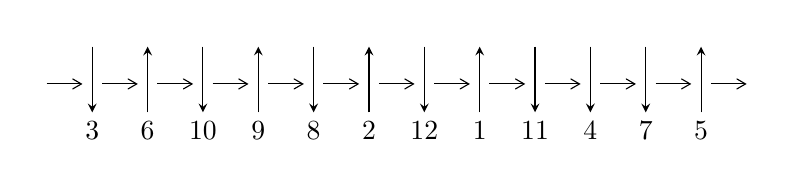
\begin{tikzpicture}[x=20pt, y=17pt]
	% nodes
	\node (C0) at (0, 0) {};
	\node (C1) at (1, 0) {};
	\node (C1U) at (1, +1) {};
	\node (C1D) at (1, -1) {3};

	\node (C2) at (2, 0) {};
	\node (C2U) at (2, +1) {};
	\node (C2D) at (2, -1) {6};

	\node (C3) at (3, 0) {};
	\node (C3U) at (3, +1) {};
	\node (C3D) at (3, -1) {10};

	\node (C4) at (4, 0) {};
	\node (C4U) at (4, +1) {};
	\node (C4D) at (4, -1) {9};

	\node (C5) at (5, 0) {};
	\node (C5U) at (5, +1) {};
	\node (C5D) at (5, -1) {8};

	\node (C6) at (6, 0) {};
	\node (C6U) at (6, +1) {};
	\node (C6D) at (6, -1) {2};

	\node (C7) at (7, 0) {};
	\node (C7U) at (7, +1) {};
	\node (C7D) at (7, -1) {12};

	\node (C8) at (8, 0) {};
	\node (C8U) at (8, +1) {};
	\node (C8D) at (8, -1) {1};

	\node (C9) at (9, 0) {};
	\node (C9U) at (9, +1) {};
	\node (C9D) at (9, -1) {11};

	\node (C10) at (10, 0) {};
	\node (C10U) at (10, +1) {};
	\node (C10D) at (10, -1) {4};

	\node (C11) at (11, 0) {};
	\node (C11U) at (11, +1) {};
	\node (C11D) at (11, -1) {7};

	\node (C12) at (12, 0) {};
	\node (C12U) at (12, +1) {};
	\node (C12D) at (12, -1) {5};
	\node (C13) at (13, 0) {};

	% arrows
	\draw[->,>={angle 60}]
	(C0) edge (C1) (C1) edge (C2) (C2) edge (C3) (C3) edge (C4) (C4) edge (C5) (C5) edge (C6) (C6) edge (C7) (C7) edge (C8) (C8) edge (C9) (C9) edge (C10) (C10) edge (C11) (C11) edge (C12) (C12) edge (C13) ;	\draw[->,>=stealth]
	(C1U) edge (C1D) (C2D) edge (C2U) (C3U) edge (C3D) (C4D) edge (C4U) (C5U) edge (C5D) (C6D) edge (C6U) (C7U) edge (C7D) (C8D) edge (C8U) (C9U) edge (C9D) (C10U) edge (C10D) (C11U) edge (C11D) (C12D) edge (C12U) ;
	\end{tikzpicture} \\
\hhline{~~} \\& 
\textbf{Solving Sequence} \\ \cline{2-2} 
 &
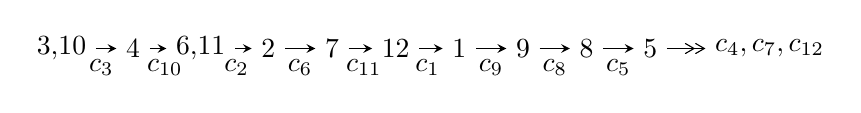
\begin{tikzpicture}[x=23pt, y=7pt]
	% node
	\node (A0) at (-1/8, 0) {3,10};
	\node (A1) at (1, 0) {4};
	\node (A2) at (33/16, 0) {6,11};
	\node (A3) at (25/8, 0) {2};
	\node (A4) at (33/8, 0) {7};
	\node (A5) at (41/8, 0) {12};
	\node (A6) at (49/8, 0) {1};
	\node (A7) at (57/8, 0) {9};
	\node (A8) at (65/8, 0) {8};
	\node (A9) at (73/8, 0) {5};
	\node (C1) at (1/2, -1) {$c_{3}$};
	\node (C2) at (3/2, -1) {$c_{10}$};
	\node (C3) at (21/8, -1) {$c_{2}$};
	\node (C4) at (29/8, -1) {$c_{6}$};
	\node (C5) at (37/8, -1) {$c_{11}$};
	\node (C6) at (45/8, -1) {$c_{1}$};
	\node (C7) at (53/8, -1) {$c_{9}$};
	\node (C8) at (61/8, -1) {$c_{8}$};
	\node (C9) at (69/8, -1) {$c_{5}$};
	\node (A10) at (11, 0) {$c_{4},c_{7},c_{12}$};

	% edge
	\draw[->,>=stealth]	
	(A0) edge (A1) (A1) edge (A2) (A2) edge (A3) (A3) edge (A4) (A4) edge (A5) (A5) edge (A6) (A6) edge (A7) (A7) edge (A8) (A8) edge (A9) ;
	\draw[->>,>={angle 60}]	
	(A9) edge (A10);
\end{tikzpicture} \\ 

\end{tabular} \\

\footnotetext{
The image of knot diagram is generated by the software ``\textbf{Draw programme}" developed by Andrew Bartholomew(\url{http://www.layer8.co.uk/maths/draw/index.htm\#Running-draw}), where we modified some parts for our purpose(\url{https://github.com/CATsTAILs/LinksPainter}).
}\phantom \\ \newline 
\centering \textbf{Ideals for irreducible components\footnotemark of $X_{\text{par}}$} 
 
\begin{align*}
I^u_{1}&=\langle 
2.15850\times10^{215} u^{141}+1.12135\times10^{215} u^{140}+\cdots+1.47358\times10^{214} b+4.27986\times10^{215},\\
\phantom{I^u_{1}}&\phantom{= \langle  }-1.02103\times10^{216} u^{141}-3.98145\times10^{215} u^{140}+\cdots+1.47358\times10^{214} a-1.65816\times10^{216},\\
\phantom{I^u_{1}}&\phantom{= \langle  }u^{142}+u^{141}+\cdots+2 u+1\rangle \\
I^u_{2}&=\langle 
-5 u^{29}+37 u^{27}+\cdots+b+1,\;u^{29}-6 u^{28}+\cdots+a+16,\;u^{30}-8 u^{28}+\cdots-6 u^2+1\rangle \\
I^u_{3}&=\langle 
- u^2+b,\;u^2+a-1,\;u^9- u^7+u^5+u-1\rangle \\
\\
\end{align*}
\raggedright * 3 irreducible components of $\dim_{\mathbb{C}}=0$, with total 181 representations.\\
\footnotetext{All coefficients of polynomials are rational numbers. But the coefficients are sometimes approximated in decimal forms when there is not enough margin.}
\newpage
\renewcommand{\arraystretch}{1}
\centering \section*{I. $I^u_{1}= \langle 2.16\times10^{215} u^{141}+1.12\times10^{215} u^{140}+\cdots+1.47\times10^{214} b+4.28\times10^{215},\;-1.02\times10^{216} u^{141}-3.98\times10^{215} u^{140}+\cdots+1.47\times10^{214} a-1.66\times10^{216},\;u^{142}+u^{141}+\cdots+2 u+1 \rangle$}
\flushleft \textbf{(i) Arc colorings}\\
\begin{tabular}{m{7pt} m{180pt} m{7pt} m{180pt} }
\flushright $a_{3}=$&$\begin{pmatrix}1\\0\end{pmatrix}$ \\
\flushright $a_{10}=$&$\begin{pmatrix}0\\u\end{pmatrix}$ \\
\flushright $a_{4}=$&$\begin{pmatrix}1\\u^2\end{pmatrix}$ \\
\flushright $a_{6}=$&$\begin{pmatrix}69.2888 u^{141}+27.0189 u^{140}+\cdots+60.3781 u+112.526\\-14.6480 u^{141}-7.60972 u^{140}+\cdots-3.77923 u-29.0439\end{pmatrix}$ \\
\flushright $a_{11}=$&$\begin{pmatrix}- u\\- u^3+u\end{pmatrix}$ \\
\flushright $a_{2}=$&$\begin{pmatrix}98.5271 u^{141}+51.8440 u^{140}+\cdots-20.6958 u+209.268\\-15.8723 u^{141}-9.69013 u^{140}+\cdots+8.74357 u-36.7595\end{pmatrix}$ \\
\flushright $a_{7}=$&$\begin{pmatrix}70.6230 u^{141}+32.6381 u^{140}+\cdots+24.8012 u+130.839\\-3.19139 u^{141}-1.99522 u^{140}+\cdots+1.36837 u-7.21709\end{pmatrix}$ \\
\flushright $a_{12}=$&$\begin{pmatrix}-105.596 u^{141}-54.7390 u^{140}+\cdots+20.3905 u-221.860\\14.8864 u^{141}+8.90364 u^{140}+\cdots-7.43228 u+33.9364\end{pmatrix}$ \\
\flushright $a_{1}=$&$\begin{pmatrix}82.6547 u^{141}+42.1539 u^{140}+\cdots-11.9522 u+172.509\\-15.8723 u^{141}-9.69013 u^{140}+\cdots+8.74357 u-36.7595\end{pmatrix}$ \\
\flushright $a_{9}=$&$\begin{pmatrix}u^3\\u^5- u^3+u\end{pmatrix}$ \\
\flushright $a_{8}=$&$\begin{pmatrix}-12.2390 u^{141}-10.0968 u^{140}+\cdots+43.9408 u-42.9882\\-12.0821 u^{141}-4.24533 u^{140}+\cdots-5.97197 u-18.4046\end{pmatrix}$ \\
\flushright $a_{5}=$&$\begin{pmatrix}u^6- u^4+1\\u^8-2 u^6+2 u^4\end{pmatrix}$\\&\end{tabular}
\flushleft \textbf{(ii) Obstruction class $= -1$}\\~\\
\flushleft \textbf{(iii) Cusp Shapes $= 5.34809 u^{141}+4.05326 u^{140}+\cdots-19.7693 u+23.7811$}\\~\\
\newpage\renewcommand{\arraystretch}{1}
\flushleft \textbf{(iv) u-Polynomials at the component}\newline \\
\begin{tabular}{m{50pt}|m{274pt}}
Crossings & \hspace{64pt}u-Polynomials at each crossing \\
\hline $$\begin{aligned}c_{1}\end{aligned}$$&$\begin{aligned}
&u^{142}+68 u^{141}+\cdots+45485023 u+1940449
\end{aligned}$\\
\hline $$\begin{aligned}c_{2},c_{6}\end{aligned}$$&$\begin{aligned}
&u^{142}-2 u^{141}+\cdots+793 u+1393
\end{aligned}$\\
\hline $$\begin{aligned}c_{3},c_{10}\end{aligned}$$&$\begin{aligned}
&u^{142}- u^{141}+\cdots-2 u+1
\end{aligned}$\\
\hline $$\begin{aligned}c_{4}\end{aligned}$$&$\begin{aligned}
&u^{142}-3 u^{141}+\cdots-3417185 u+423016
\end{aligned}$\\
\hline $$\begin{aligned}c_{5}\end{aligned}$$&$\begin{aligned}
&u^{142}-9 u^{141}+\cdots-48 u+1
\end{aligned}$\\
\hline $$\begin{aligned}c_{7},c_{11}\end{aligned}$$&$\begin{aligned}
&u^{142}-10 u^{141}+\cdots-1373392 u+119344
\end{aligned}$\\
\hline $$\begin{aligned}c_{8}\end{aligned}$$&$\begin{aligned}
&u^{142}-5 u^{141}+\cdots+1486 u+347
\end{aligned}$\\
\hline $$\begin{aligned}c_{9}\end{aligned}$$&$\begin{aligned}
&u^{142}+75 u^{141}+\cdots+12 u+1
\end{aligned}$\\
\hline $$\begin{aligned}c_{12}\end{aligned}$$&$\begin{aligned}
&u^{142}- u^{141}+\cdots-68944 u+61373
\end{aligned}$\\
\hline
\end{tabular}\\~\\
\newpage\renewcommand{\arraystretch}{1}
\flushleft \textbf{(v) Riley Polynomials at the component}\newline \\
\begin{tabular}{m{50pt}|m{274pt}}
Crossings & \hspace{64pt}Riley Polynomials at each crossing \\
\hline $$\begin{aligned}c_{1}\end{aligned}$$&$\begin{aligned}
&y^{142}+28 y^{141}+\cdots+136799040774219 y+3765342321601
\end{aligned}$\\
\hline $$\begin{aligned}c_{2},c_{6}\end{aligned}$$&$\begin{aligned}
&y^{142}+68 y^{141}+\cdots+45485023 y+1940449
\end{aligned}$\\
\hline $$\begin{aligned}c_{3},c_{10}\end{aligned}$$&$\begin{aligned}
&y^{142}-75 y^{141}+\cdots-12 y+1
\end{aligned}$\\
\hline $$\begin{aligned}c_{4}\end{aligned}$$&$\begin{aligned}
&y^{142}+81 y^{141}+\cdots-614480347793 y+178942536256
\end{aligned}$\\
\hline $$\begin{aligned}c_{5}\end{aligned}$$&$\begin{aligned}
&y^{142}-11 y^{141}+\cdots-96 y+1
\end{aligned}$\\
\hline $$\begin{aligned}c_{7},c_{11}\end{aligned}$$&$\begin{aligned}
&y^{142}-98 y^{141}+\cdots-733475256192 y+14242990336
\end{aligned}$\\
\hline $$\begin{aligned}c_{8}\end{aligned}$$&$\begin{aligned}
&y^{142}+17 y^{141}+\cdots+8068556 y+120409
\end{aligned}$\\
\hline $$\begin{aligned}c_{9}\end{aligned}$$&$\begin{aligned}
&y^{142}-3 y^{141}+\cdots-56 y+1
\end{aligned}$\\
\hline $$\begin{aligned}c_{12}\end{aligned}$$&$\begin{aligned}
&y^{142}+37 y^{141}+\cdots+186760312142 y+3766645129
\end{aligned}$\\
\hline
\end{tabular}\\~\\
\newpage\flushleft \textbf{(vi) Complex Volumes and Cusp Shapes}
$$\begin{array}{c|c|c}  
\text{Solutions to }I^u_{1}& \I (\text{vol} + \sqrt{-1}CS) & \text{Cusp shape}\\
 \hline 
\begin{aligned}
u &= \phantom{-}0.819925 + 0.573197 I \\
a &= \phantom{-}0.879246 + 0.964168 I \\
b &= -0.686532 - 0.919738 I\end{aligned}
 & \phantom{-}2.90346 + 1.92369 I & \phantom{-0.000000 } 0 \\ \hline\begin{aligned}
u &= \phantom{-}0.819925 - 0.573197 I \\
a &= \phantom{-}0.879246 - 0.964168 I \\
b &= -0.686532 + 0.919738 I\end{aligned}
 & \phantom{-}2.90346 - 1.92369 I & \phantom{-0.000000 } 0 \\ \hline\begin{aligned}
u &= -0.998317 + 0.162663 I \\
a &= \phantom{-}0.15234 + 1.72026 I \\
b &= \phantom{-}0.429286 + 0.749945 I\end{aligned}
 & -1.98733 + 4.15694 I & \phantom{-0.000000 } 0 \\ \hline\begin{aligned}
u &= -0.998317 - 0.162663 I \\
a &= \phantom{-}0.15234 - 1.72026 I \\
b &= \phantom{-}0.429286 - 0.749945 I\end{aligned}
 & -1.98733 - 4.15694 I & \phantom{-0.000000 } 0 \\ \hline\begin{aligned}
u &= \phantom{-}0.983094 + 0.270642 I \\
a &= \phantom{-}0.329558 + 0.164084 I \\
b &= \phantom{-}0.379901 + 0.532584 I\end{aligned}
 & -1.85848 - 0.87645 I & \phantom{-0.000000 } 0 \\ \hline\begin{aligned}
u &= \phantom{-}0.983094 - 0.270642 I \\
a &= \phantom{-}0.329558 - 0.164084 I \\
b &= \phantom{-}0.379901 - 0.532584 I\end{aligned}
 & -1.85848 + 0.87645 I & \phantom{-0.000000 } 0 \\ \hline\begin{aligned}
u &= -0.336460 + 0.966769 I \\
a &= \phantom{-}1.40956 - 0.63858 I \\
b &= -0.552563 + 1.026870 I\end{aligned}
 & -3.12233 - 4.55892 I & \phantom{-0.000000 } 0 \\ \hline\begin{aligned}
u &= -0.336460 - 0.966769 I \\
a &= \phantom{-}1.40956 + 0.63858 I \\
b &= -0.552563 - 1.026870 I\end{aligned}
 & -3.12233 + 4.55892 I & \phantom{-0.000000 } 0 \\ \hline\begin{aligned}
u &= \phantom{-}0.769689 + 0.689370 I \\
a &= -1.24009 - 0.71557 I \\
b &= \phantom{-}0.760360 + 0.502335 I\end{aligned}
 & \phantom{-}1.41703 - 6.24375 I & \phantom{-0.000000 } 0 \\ \hline\begin{aligned}
u &= \phantom{-}0.769689 - 0.689370 I \\
a &= -1.24009 + 0.71557 I \\
b &= \phantom{-}0.760360 - 0.502335 I\end{aligned}
 & \phantom{-}1.41703 + 6.24375 I & \phantom{-0.000000 } 0\\
 \hline 
 \end{array}$$\newpage$$\begin{array}{c|c|c}  
\text{Solutions to }I^u_{1}& \I (\text{vol} + \sqrt{-1}CS) & \text{Cusp shape}\\
 \hline 
\begin{aligned}
u &= \phantom{-}0.752662 + 0.593812 I \\
a &= -2.39364 - 0.09867 I \\
b &= \phantom{-}0.661817 - 0.973208 I\end{aligned}
 & \phantom{-}3.09116 - 6.54197 I & \phantom{-0.000000 } 0 \\ \hline\begin{aligned}
u &= \phantom{-}0.752662 - 0.593812 I \\
a &= -2.39364 + 0.09867 I \\
b &= \phantom{-}0.661817 + 0.973208 I\end{aligned}
 & \phantom{-}3.09116 + 6.54197 I & \phantom{-0.000000 } 0 \\ \hline\begin{aligned}
u &= -0.102308 + 1.037670 I \\
a &= \phantom{-}0.804635 + 0.252765 I \\
b &= -0.341980 - 0.947064 I\end{aligned}
 & -4.69706 + 1.29869 I & \phantom{-0.000000 } 0 \\ \hline\begin{aligned}
u &= -0.102308 - 1.037670 I \\
a &= \phantom{-}0.804635 - 0.252765 I \\
b &= -0.341980 + 0.947064 I\end{aligned}
 & -4.69706 - 1.29869 I & \phantom{-0.000000 } 0 \\ \hline\begin{aligned}
u &= -0.886405 + 0.577385 I \\
a &= \phantom{-}1.92287 + 0.05036 I \\
b &= -0.710853 - 0.743340 I\end{aligned}
 & \phantom{-}3.41659 + 3.40993 I & \phantom{-0.000000 } 0 \\ \hline\begin{aligned}
u &= -0.886405 - 0.577385 I \\
a &= \phantom{-}1.92287 - 0.05036 I \\
b &= -0.710853 + 0.743340 I\end{aligned}
 & \phantom{-}3.41659 - 3.40993 I & \phantom{-0.000000 } 0 \\ \hline\begin{aligned}
u &= \phantom{-}0.827768 + 0.692948 I \\
a &= \phantom{-}1.78087 + 0.30538 I \\
b &= -0.626794 + 0.564260 I\end{aligned}
 & \phantom{-}1.26246 + 1.00442 I & \phantom{-0.000000 } 0 \\ \hline\begin{aligned}
u &= \phantom{-}0.827768 - 0.692948 I \\
a &= \phantom{-}1.78087 - 0.30538 I \\
b &= -0.626794 - 0.564260 I\end{aligned}
 & \phantom{-}1.26246 - 1.00442 I & \phantom{-0.000000 } 0 \\ \hline\begin{aligned}
u &= -0.262097 + 0.881582 I \\
a &= -1.56596 + 0.44079 I \\
b &= \phantom{-}0.647747 - 1.172540 I\end{aligned}
 & -3.7320 - 14.3288 I & \phantom{-0.000000 } 0 \\ \hline\begin{aligned}
u &= -0.262097 - 0.881582 I \\
a &= -1.56596 - 0.44079 I \\
b &= \phantom{-}0.647747 + 1.172540 I\end{aligned}
 & -3.7320 + 14.3288 I & \phantom{-0.000000 } 0\\
 \hline 
 \end{array}$$\newpage$$\begin{array}{c|c|c}  
\text{Solutions to }I^u_{1}& \I (\text{vol} + \sqrt{-1}CS) & \text{Cusp shape}\\
 \hline 
\begin{aligned}
u &= -0.675824 + 0.615061 I \\
a &= -0.95501 + 1.31977 I \\
b &= \phantom{-}0.714573 - 0.655402 I\end{aligned}
 & \phantom{-}4.02613 + 1.27883 I & \phantom{-0.000000 } 0 \\ \hline\begin{aligned}
u &= -0.675824 - 0.615061 I \\
a &= -0.95501 - 1.31977 I \\
b &= \phantom{-}0.714573 + 0.655402 I\end{aligned}
 & \phantom{-}4.02613 - 1.27883 I & \phantom{-0.000000 } 0 \\ \hline\begin{aligned}
u &= \phantom{-}0.981739 + 0.467961 I \\
a &= -0.83111 + 2.10000 I \\
b &= -0.290470 - 0.855232 I\end{aligned}
 & -4.11806 + 0.96122 I & \phantom{-0.000000 } 0 \\ \hline\begin{aligned}
u &= \phantom{-}0.981739 - 0.467961 I \\
a &= -0.83111 - 2.10000 I \\
b &= -0.290470 + 0.855232 I\end{aligned}
 & -4.11806 - 0.96122 I & \phantom{-0.000000 } 0 \\ \hline\begin{aligned}
u &= -1.061260 + 0.329465 I \\
a &= \phantom{-}0.516163 - 1.058550 I \\
b &= \phantom{-}0.471837 - 1.310330 I\end{aligned}
 & -5.43261 - 3.34267 I & \phantom{-0.000000 } 0 \\ \hline\begin{aligned}
u &= -1.061260 - 0.329465 I \\
a &= \phantom{-}0.516163 + 1.058550 I \\
b &= \phantom{-}0.471837 + 1.310330 I\end{aligned}
 & -5.43261 + 3.34267 I & \phantom{-0.000000 } 0 \\ \hline\begin{aligned}
u &= -0.825572 + 0.325567 I \\
a &= -0.102107 - 0.515957 I \\
b &= -0.239822 - 1.224430 I\end{aligned}
 & -4.72518 + 5.65170 I & \phantom{-0.000000 } 0 \\ \hline\begin{aligned}
u &= -0.825572 - 0.325567 I \\
a &= -0.102107 + 0.515957 I \\
b &= -0.239822 + 1.224430 I\end{aligned}
 & -4.72518 - 5.65170 I & \phantom{-0.000000 } 0 \\ \hline\begin{aligned}
u &= -0.835490 + 0.753017 I \\
a &= -1.91088 - 0.30285 I \\
b &= \phantom{-}0.606604 + 1.064330 I\end{aligned}
 & -0.26999 + 11.42200 I & \phantom{-0.000000 } 0 \\ \hline\begin{aligned}
u &= -0.835490 - 0.753017 I \\
a &= -1.91088 + 0.30285 I \\
b &= \phantom{-}0.606604 - 1.064330 I\end{aligned}
 & -0.26999 - 11.42200 I & \phantom{-0.000000 } 0\\
 \hline 
 \end{array}$$\newpage$$\begin{array}{c|c|c}  
\text{Solutions to }I^u_{1}& \I (\text{vol} + \sqrt{-1}CS) & \text{Cusp shape}\\
 \hline 
\begin{aligned}
u &= -0.796220 + 0.800451 I \\
a &= \phantom{-}0.638727 - 0.980874 I \\
b &= -0.560690 + 1.022220 I\end{aligned}
 & -0.12297 - 5.68905 I & \phantom{-0.000000 } 0 \\ \hline\begin{aligned}
u &= -0.796220 - 0.800451 I \\
a &= \phantom{-}0.638727 + 0.980874 I \\
b &= -0.560690 - 1.022220 I\end{aligned}
 & -0.12297 + 5.68905 I & \phantom{-0.000000 } 0 \\ \hline\begin{aligned}
u &= \phantom{-}0.265127 + 0.826576 I \\
a &= -1.42559 + 0.49190 I \\
b &= \phantom{-}0.950982 - 0.387299 I\end{aligned}
 & -1.32824 + 8.51203 I & \phantom{-0.000000 } 0 \\ \hline\begin{aligned}
u &= \phantom{-}0.265127 - 0.826576 I \\
a &= -1.42559 - 0.49190 I \\
b &= \phantom{-}0.950982 + 0.387299 I\end{aligned}
 & -1.32824 - 8.51203 I & \phantom{-0.000000 } 0 \\ \hline\begin{aligned}
u &= \phantom{-}1.038220 + 0.468696 I \\
a &= \phantom{-}0.143061 - 0.914417 I \\
b &= \phantom{-}0.907283 + 0.353856 I\end{aligned}
 & -0.461214 - 1.205920 I & \phantom{-0.000000 } 0 \\ \hline\begin{aligned}
u &= \phantom{-}1.038220 - 0.468696 I \\
a &= \phantom{-}0.143061 + 0.914417 I \\
b &= \phantom{-}0.907283 - 0.353856 I\end{aligned}
 & -0.461214 + 1.205920 I & \phantom{-0.000000 } 0 \\ \hline\begin{aligned}
u &= \phantom{-}0.357950 + 0.775515 I \\
a &= \phantom{-}1.41875 + 0.05983 I \\
b &= -0.335547 - 0.925700 I\end{aligned}
 & -1.48529 + 2.74039 I & \phantom{-0.000000 } 0 \\ \hline\begin{aligned}
u &= \phantom{-}0.357950 - 0.775515 I \\
a &= \phantom{-}1.41875 - 0.05983 I \\
b &= -0.335547 + 0.925700 I\end{aligned}
 & -1.48529 - 2.74039 I & \phantom{-0.000000 } 0 \\ \hline\begin{aligned}
u &= -1.120770 + 0.262113 I \\
a &= -0.22224 - 1.55747 I \\
b &= \phantom{-}0.165035 - 1.029870 I\end{aligned}
 & -5.95469 - 0.06109 I & \phantom{-0.000000 } 0 \\ \hline\begin{aligned}
u &= -1.120770 - 0.262113 I \\
a &= -0.22224 + 1.55747 I \\
b &= \phantom{-}0.165035 + 1.029870 I\end{aligned}
 & -5.95469 + 0.06109 I & \phantom{-0.000000 } 0\\
 \hline 
 \end{array}$$\newpage$$\begin{array}{c|c|c}  
\text{Solutions to }I^u_{1}& \I (\text{vol} + \sqrt{-1}CS) & \text{Cusp shape}\\
 \hline 
\begin{aligned}
u &= \phantom{-}1.120430 + 0.285920 I \\
a &= \phantom{-}0.030486 + 0.400743 I \\
b &= -0.547562 + 0.446101 I\end{aligned}
 & -1.94419 + 0.00486 I & \phantom{-0.000000 } 0 \\ \hline\begin{aligned}
u &= \phantom{-}1.120430 - 0.285920 I \\
a &= \phantom{-}0.030486 - 0.400743 I \\
b &= -0.547562 - 0.446101 I\end{aligned}
 & -1.94419 - 0.00486 I & \phantom{-0.000000 } 0 \\ \hline\begin{aligned}
u &= \phantom{-}0.587273 + 0.586722 I \\
a &= \phantom{-}1.68540 - 0.81948 I \\
b &= -0.631334 + 1.116390 I\end{aligned}
 & -0.58161 - 4.44960 I & \phantom{-0.000000 -}0. + 7.84954 I \\ \hline\begin{aligned}
u &= \phantom{-}0.587273 - 0.586722 I \\
a &= \phantom{-}1.68540 + 0.81948 I \\
b &= -0.631334 - 1.116390 I\end{aligned}
 & -0.58161 + 4.44960 I & \phantom{-0.000000 } 0. - 7.84954 I \\ \hline\begin{aligned}
u &= -1.058660 + 0.516485 I \\
a &= -0.598797 + 1.113080 I \\
b &= \phantom{-}0.876245 - 0.001895 I\end{aligned}
 & \phantom{-}0.01537 + 5.05199 I & \phantom{-0.000000 } 0 \\ \hline\begin{aligned}
u &= -1.058660 - 0.516485 I \\
a &= -0.598797 - 1.113080 I \\
b &= \phantom{-}0.876245 + 0.001895 I\end{aligned}
 & \phantom{-}0.01537 - 5.05199 I & \phantom{-0.000000 } 0 \\ \hline\begin{aligned}
u &= \phantom{-}0.219678 + 0.781394 I \\
a &= -1.59503 + 0.21320 I \\
b &= \phantom{-}0.582661 + 1.058010 I\end{aligned}
 & \phantom{-}0.56062 + 7.88617 I & -2.00000 - 7.64027 I \\ \hline\begin{aligned}
u &= \phantom{-}0.219678 - 0.781394 I \\
a &= -1.59503 - 0.21320 I \\
b &= \phantom{-}0.582661 - 1.058010 I\end{aligned}
 & \phantom{-}0.56062 - 7.88617 I & -2.00000 + 7.64027 I \\ \hline\begin{aligned}
u &= -0.810891 + 0.018995 I \\
a &= -0.44839 + 2.20459 I \\
b &= \phantom{-}0.442563 + 1.132130 I\end{aligned}
 & -4.66414 + 3.91640 I & -11.24169 + 0. I\phantom{ +0.000000I} \\ \hline\begin{aligned}
u &= -0.810891 - 0.018995 I \\
a &= -0.44839 - 2.20459 I \\
b &= \phantom{-}0.442563 - 1.132130 I\end{aligned}
 & -4.66414 - 3.91640 I & -11.24169 + 0. I\phantom{ +0.000000I}\\
 \hline 
 \end{array}$$\newpage$$\begin{array}{c|c|c}  
\text{Solutions to }I^u_{1}& \I (\text{vol} + \sqrt{-1}CS) & \text{Cusp shape}\\
 \hline 
\begin{aligned}
u &= -1.106370 + 0.437420 I \\
a &= \phantom{-}2.29478 - 2.07878 I \\
b &= -0.380770 - 0.983522 I\end{aligned}
 & -4.77162 + 1.80859 I & \phantom{-0.000000 } 0 \\ \hline\begin{aligned}
u &= -1.106370 - 0.437420 I \\
a &= \phantom{-}2.29478 + 2.07878 I \\
b &= -0.380770 + 0.983522 I\end{aligned}
 & -4.77162 - 1.80859 I & \phantom{-0.000000 } 0 \\ \hline\begin{aligned}
u &= -1.061380 + 0.538697 I \\
a &= -1.18916 + 0.82215 I \\
b &= \phantom{-}0.782131 + 0.441989 I\end{aligned}
 & -0.10586 + 5.44582 I & \phantom{-0.000000 } 0 \\ \hline\begin{aligned}
u &= -1.061380 - 0.538697 I \\
a &= -1.18916 - 0.82215 I \\
b &= \phantom{-}0.782131 - 0.441989 I\end{aligned}
 & -0.10586 - 5.44582 I & \phantom{-0.000000 } 0 \\ \hline\begin{aligned}
u &= -1.124720 + 0.396145 I \\
a &= \phantom{-}0.693007 + 0.740985 I \\
b &= -0.539884 + 1.115230 I\end{aligned}
 & -7.31755 - 1.87859 I & \phantom{-0.000000 } 0 \\ \hline\begin{aligned}
u &= -1.124720 - 0.396145 I \\
a &= \phantom{-}0.693007 - 0.740985 I \\
b &= -0.539884 - 1.115230 I\end{aligned}
 & -7.31755 + 1.87859 I & \phantom{-0.000000 } 0 \\ \hline\begin{aligned}
u &= \phantom{-}1.120490 + 0.414286 I \\
a &= \phantom{-}0.431652 + 0.605235 I \\
b &= \phantom{-}0.452609 + 1.065390 I\end{aligned}
 & -3.01714 - 0.96511 I & \phantom{-0.000000 } 0 \\ \hline\begin{aligned}
u &= \phantom{-}1.120490 - 0.414286 I \\
a &= \phantom{-}0.431652 - 0.605235 I \\
b &= \phantom{-}0.452609 - 1.065390 I\end{aligned}
 & -3.01714 + 0.96511 I & \phantom{-0.000000 } 0 \\ \hline\begin{aligned}
u &= \phantom{-}1.101160 + 0.477897 I \\
a &= -1.59513 - 0.83858 I \\
b &= \phantom{-}1.065770 - 0.832707 I\end{aligned}
 & -1.30656 - 7.29187 I & \phantom{-0.000000 } 0 \\ \hline\begin{aligned}
u &= \phantom{-}1.101160 - 0.477897 I \\
a &= -1.59513 + 0.83858 I \\
b &= \phantom{-}1.065770 + 0.832707 I\end{aligned}
 & -1.30656 + 7.29187 I & \phantom{-0.000000 } 0\\
 \hline 
 \end{array}$$\newpage$$\begin{array}{c|c|c}  
\text{Solutions to }I^u_{1}& \I (\text{vol} + \sqrt{-1}CS) & \text{Cusp shape}\\
 \hline 
\begin{aligned}
u &= -0.146851 + 0.783292 I \\
a &= -0.306003 - 0.486855 I \\
b &= \phantom{-}0.100720 + 1.339030 I\end{aligned}
 & -7.52306 - 5.15147 I & -7.08476 + 4.50382 I \\ \hline\begin{aligned}
u &= -0.146851 - 0.783292 I \\
a &= -0.306003 + 0.486855 I \\
b &= \phantom{-}0.100720 - 1.339030 I\end{aligned}
 & -7.52306 + 5.15147 I & -7.08476 - 4.50382 I \\ \hline\begin{aligned}
u &= -1.118420 + 0.447051 I \\
a &= \phantom{-}0.38796 - 1.51839 I \\
b &= -0.672384 + 0.533733 I\end{aligned}
 & -5.05939 + 4.74367 I & \phantom{-0.000000 } 0 \\ \hline\begin{aligned}
u &= -1.118420 - 0.447051 I \\
a &= \phantom{-}0.38796 + 1.51839 I \\
b &= -0.672384 - 0.533733 I\end{aligned}
 & -5.05939 - 4.74367 I & \phantom{-0.000000 } 0 \\ \hline\begin{aligned}
u &= -0.284485 + 0.740309 I \\
a &= -0.781132 - 0.751379 I \\
b &= \phantom{-}0.692387 + 0.481448 I\end{aligned}
 & \phantom{-}2.26299 - 2.95719 I & \phantom{-}2.44235 + 2.41736 I \\ \hline\begin{aligned}
u &= -0.284485 - 0.740309 I \\
a &= -0.781132 + 0.751379 I \\
b &= \phantom{-}0.692387 - 0.481448 I\end{aligned}
 & \phantom{-}2.26299 + 2.95719 I & \phantom{-}2.44235 - 2.41736 I \\ \hline\begin{aligned}
u &= \phantom{-}1.115220 + 0.468441 I \\
a &= -0.55244 - 1.56579 I \\
b &= -0.242606 - 1.060950 I\end{aligned}
 & -4.53390 - 5.70007 I & \phantom{-0.000000 } 0 \\ \hline\begin{aligned}
u &= \phantom{-}1.115220 - 0.468441 I \\
a &= -0.55244 + 1.56579 I \\
b &= -0.242606 + 1.060950 I\end{aligned}
 & -4.53390 + 5.70007 I & \phantom{-0.000000 } 0 \\ \hline\begin{aligned}
u &= \phantom{-}0.044027 + 0.788764 I \\
a &= \phantom{-}0.147867 - 0.134067 I \\
b &= \phantom{-}0.327426 - 0.992104 I\end{aligned}
 & -5.35872 - 1.03966 I & -10.97184 + 1.37054 I \\ \hline\begin{aligned}
u &= \phantom{-}0.044027 - 0.788764 I \\
a &= \phantom{-}0.147867 + 0.134067 I \\
b &= \phantom{-}0.327426 + 0.992104 I\end{aligned}
 & -5.35872 + 1.03966 I & -10.97184 - 1.37054 I\\
 \hline 
 \end{array}$$\newpage$$\begin{array}{c|c|c}  
\text{Solutions to }I^u_{1}& \I (\text{vol} + \sqrt{-1}CS) & \text{Cusp shape}\\
 \hline 
\begin{aligned}
u &= \phantom{-}1.124070 + 0.450929 I \\
a &= \phantom{-}0.582151 - 0.061219 I \\
b &= -0.719681 + 0.339253 I\end{aligned}
 & -5.01892 - 2.92665 I & \phantom{-0.000000 } 0 \\ \hline\begin{aligned}
u &= \phantom{-}1.124070 - 0.450929 I \\
a &= \phantom{-}0.582151 + 0.061219 I \\
b &= -0.719681 - 0.339253 I\end{aligned}
 & -5.01892 + 2.92665 I & \phantom{-0.000000 } 0 \\ \hline\begin{aligned}
u &= -1.030980 + 0.639248 I \\
a &= -0.066615 + 0.964674 I \\
b &= \phantom{-}0.256363 - 0.901271 I\end{aligned}
 & -3.06581 + 5.46183 I & \phantom{-0.000000 } 0 \\ \hline\begin{aligned}
u &= -1.030980 - 0.639248 I \\
a &= -0.066615 - 0.964674 I \\
b &= \phantom{-}0.256363 + 0.901271 I\end{aligned}
 & -3.06581 - 5.46183 I & \phantom{-0.000000 } 0 \\ \hline\begin{aligned}
u &= -1.183630 + 0.278653 I \\
a &= -0.862551 + 0.065500 I \\
b &= \phantom{-}0.645704 + 0.218716 I\end{aligned}
 & -6.27261 + 3.16463 I & \phantom{-0.000000 } 0 \\ \hline\begin{aligned}
u &= -1.183630 - 0.278653 I \\
a &= -0.862551 - 0.065500 I \\
b &= \phantom{-}0.645704 - 0.218716 I\end{aligned}
 & -6.27261 - 3.16463 I & \phantom{-0.000000 } 0 \\ \hline\begin{aligned}
u &= -1.127760 + 0.468002 I \\
a &= -1.73382 + 1.41012 I \\
b &= \phantom{-}0.627158 + 1.114120 I\end{aligned}
 & -2.64743 + 6.77904 I & \phantom{-0.000000 } 0 \\ \hline\begin{aligned}
u &= -1.127760 - 0.468002 I \\
a &= -1.73382 - 1.41012 I \\
b &= \phantom{-}0.627158 - 1.114120 I\end{aligned}
 & -2.64743 - 6.77904 I & \phantom{-0.000000 } 0 \\ \hline\begin{aligned}
u &= -1.182600 + 0.328583 I \\
a &= \phantom{-}0.040553 + 1.247040 I \\
b &= -0.523046 + 1.043670 I\end{aligned}
 & -3.66226 - 4.36716 I & \phantom{-0.000000 } 0 \\ \hline\begin{aligned}
u &= -1.182600 - 0.328583 I \\
a &= \phantom{-}0.040553 - 1.247040 I \\
b &= -0.523046 - 1.043670 I\end{aligned}
 & -3.66226 + 4.36716 I & \phantom{-0.000000 } 0\\
 \hline 
 \end{array}$$\newpage$$\begin{array}{c|c|c}  
\text{Solutions to }I^u_{1}& \I (\text{vol} + \sqrt{-1}CS) & \text{Cusp shape}\\
 \hline 
\begin{aligned}
u &= \phantom{-}1.112390 + 0.534778 I \\
a &= -2.25516 - 1.06311 I \\
b &= \phantom{-}0.61062 - 1.32428 I\end{aligned}
 & -3.95389 - 10.65120 I & \phantom{-0.000000 } 0 \\ \hline\begin{aligned}
u &= \phantom{-}1.112390 - 0.534778 I \\
a &= -2.25516 + 1.06311 I \\
b &= \phantom{-}0.61062 + 1.32428 I\end{aligned}
 & -3.95389 + 10.65120 I & \phantom{-0.000000 } 0 \\ \hline\begin{aligned}
u &= \phantom{-}1.132030 + 0.495273 I \\
a &= \phantom{-}2.78786 + 0.82100 I \\
b &= -0.586312 + 1.047710 I\end{aligned}
 & -6.60530 - 9.65736 I & \phantom{-0.000000 } 0 \\ \hline\begin{aligned}
u &= \phantom{-}1.132030 - 0.495273 I \\
a &= \phantom{-}2.78786 - 0.82100 I \\
b &= -0.586312 - 1.047710 I\end{aligned}
 & -6.60530 + 9.65736 I & \phantom{-0.000000 } 0 \\ \hline\begin{aligned}
u &= -1.206510 + 0.271984 I \\
a &= \phantom{-}0.438591 - 0.468643 I \\
b &= -0.927115 - 0.288564 I\end{aligned}
 & -6.00510 - 5.09569 I & \phantom{-0.000000 } 0 \\ \hline\begin{aligned}
u &= -1.206510 - 0.271984 I \\
a &= \phantom{-}0.438591 + 0.468643 I \\
b &= -0.927115 + 0.288564 I\end{aligned}
 & -6.00510 + 5.09569 I & \phantom{-0.000000 } 0 \\ \hline\begin{aligned}
u &= -0.420856 + 0.623086 I \\
a &= \phantom{-}1.302530 - 0.322364 I \\
b &= -0.732698 + 0.315993 I\end{aligned}
 & \phantom{-}1.74958 - 0.85826 I & \phantom{-}4.53301 - 0.84557 I \\ \hline\begin{aligned}
u &= -0.420856 - 0.623086 I \\
a &= \phantom{-}1.302530 + 0.322364 I \\
b &= -0.732698 - 0.315993 I\end{aligned}
 & \phantom{-}1.74958 + 0.85826 I & \phantom{-}4.53301 + 0.84557 I \\ \hline\begin{aligned}
u &= \phantom{-}0.316242 + 0.681335 I \\
a &= \phantom{-}1.51703 + 0.62075 I \\
b &= -0.599099 - 1.263720 I\end{aligned}
 & -1.64838 + 5.95849 I & -1.86023 - 9.97228 I \\ \hline\begin{aligned}
u &= \phantom{-}0.316242 - 0.681335 I \\
a &= \phantom{-}1.51703 - 0.62075 I \\
b &= -0.599099 + 1.263720 I\end{aligned}
 & -1.64838 - 5.95849 I & -1.86023 + 9.97228 I\\
 \hline 
 \end{array}$$\newpage$$\begin{array}{c|c|c}  
\text{Solutions to }I^u_{1}& \I (\text{vol} + \sqrt{-1}CS) & \text{Cusp shape}\\
 \hline 
\begin{aligned}
u &= \phantom{-}1.204550 + 0.360848 I \\
a &= \phantom{-}1.10979 + 1.04467 I \\
b &= -0.192669 + 1.340680 I\end{aligned}
 & -11.58090 + 1.28812 I & \phantom{-0.000000 } 0 \\ \hline\begin{aligned}
u &= \phantom{-}1.204550 - 0.360848 I \\
a &= \phantom{-}1.10979 - 1.04467 I \\
b &= -0.192669 - 1.340680 I\end{aligned}
 & -11.58090 - 1.28812 I & \phantom{-0.000000 } 0 \\ \hline\begin{aligned}
u &= -1.134450 + 0.543154 I \\
a &= -0.123964 - 0.975497 I \\
b &= -0.722111 + 0.415523 I\end{aligned}
 & -0.21897 + 7.80995 I & \phantom{-0.000000 } 0 \\ \hline\begin{aligned}
u &= -1.134450 - 0.543154 I \\
a &= -0.123964 + 0.975497 I \\
b &= -0.722111 - 0.415523 I\end{aligned}
 & -0.21897 - 7.80995 I & \phantom{-0.000000 } 0 \\ \hline\begin{aligned}
u &= -0.435709 + 0.592879 I \\
a &= \phantom{-}1.350760 + 0.182256 I \\
b &= -0.785767 - 0.088874 I\end{aligned}
 & \phantom{-}1.83512 - 0.62347 I & \phantom{-}6.22978 + 1.16653 I \\ \hline\begin{aligned}
u &= -0.435709 - 0.592879 I \\
a &= \phantom{-}1.350760 - 0.182256 I \\
b &= -0.785767 + 0.088874 I\end{aligned}
 & \phantom{-}1.83512 + 0.62347 I & \phantom{-}6.22978 - 1.16653 I \\ \hline\begin{aligned}
u &= \phantom{-}1.133490 + 0.572512 I \\
a &= -2.03687 - 0.98690 I \\
b &= \phantom{-}0.365310 - 1.019860 I\end{aligned}
 & -3.80710 - 7.83125 I & \phantom{-0.000000 } 0 \\ \hline\begin{aligned}
u &= \phantom{-}1.133490 - 0.572512 I \\
a &= -2.03687 + 0.98690 I \\
b &= \phantom{-}0.365310 + 1.019860 I\end{aligned}
 & -3.80710 + 7.83125 I & \phantom{-0.000000 } 0 \\ \hline\begin{aligned}
u &= \phantom{-}0.578025 + 0.442992 I \\
a &= -2.22702 + 2.71668 I \\
b &= \phantom{-}0.418703 - 0.936982 I\end{aligned}
 & -2.89762 - 4.84473 I & -4.45896 + 8.40432 I \\ \hline\begin{aligned}
u &= \phantom{-}0.578025 - 0.442992 I \\
a &= -2.22702 - 2.71668 I \\
b &= \phantom{-}0.418703 + 0.936982 I\end{aligned}
 & -2.89762 + 4.84473 I & -4.45896 - 8.40432 I\\
 \hline 
 \end{array}$$\newpage$$\begin{array}{c|c|c}  
\text{Solutions to }I^u_{1}& \I (\text{vol} + \sqrt{-1}CS) & \text{Cusp shape}\\
 \hline 
\begin{aligned}
u &= \phantom{-}0.638347 + 0.344624 I \\
a &= \phantom{-}1.128900 + 0.503530 I \\
b &= -0.038917 + 0.902501 I\end{aligned}
 & -1.20928 - 1.53546 I & -3.16332 + 5.13059 I \\ \hline\begin{aligned}
u &= \phantom{-}0.638347 - 0.344624 I \\
a &= \phantom{-}1.128900 - 0.503530 I \\
b &= -0.038917 - 0.902501 I\end{aligned}
 & -1.20928 + 1.53546 I & -3.16332 - 5.13059 I \\ \hline\begin{aligned}
u &= \phantom{-}1.268260 + 0.172146 I \\
a &= -0.550571 + 0.487520 I \\
b &= \phantom{-}0.470552 + 1.105120 I\end{aligned}
 & -8.85021 + 1.09012 I & \phantom{-0.000000 } 0 \\ \hline\begin{aligned}
u &= \phantom{-}1.268260 - 0.172146 I \\
a &= -0.550571 - 0.487520 I \\
b &= \phantom{-}0.470552 - 1.105120 I\end{aligned}
 & -8.85021 - 1.09012 I & \phantom{-0.000000 } 0 \\ \hline\begin{aligned}
u &= -1.203140 + 0.436543 I \\
a &= \phantom{-}0.46505 - 1.38480 I \\
b &= -0.302401 - 1.041580 I\end{aligned}
 & -9.00666 + 5.34263 I & \phantom{-0.000000 } 0 \\ \hline\begin{aligned}
u &= -1.203140 - 0.436543 I \\
a &= \phantom{-}0.46505 + 1.38480 I \\
b &= -0.302401 + 1.041580 I\end{aligned}
 & -9.00666 - 5.34263 I & \phantom{-0.000000 } 0 \\ \hline\begin{aligned}
u &= -1.177010 + 0.511932 I \\
a &= -1.056080 + 0.529663 I \\
b &= -0.096574 + 1.406160 I\end{aligned}
 & -10.5281 + 9.9181 I & \phantom{-0.000000 } 0 \\ \hline\begin{aligned}
u &= -1.177010 - 0.511932 I \\
a &= -1.056080 - 0.529663 I \\
b &= -0.096574 - 1.406160 I\end{aligned}
 & -10.5281 - 9.9181 I & \phantom{-0.000000 } 0 \\ \hline\begin{aligned}
u &= \phantom{-}1.166720 + 0.535906 I \\
a &= \phantom{-}2.03104 + 1.48485 I \\
b &= -0.578682 + 1.093820 I\end{aligned}
 & -2.21982 - 12.79480 I & \phantom{-0.000000 } 0 \\ \hline\begin{aligned}
u &= \phantom{-}1.166720 - 0.535906 I \\
a &= \phantom{-}2.03104 - 1.48485 I \\
b &= -0.578682 - 1.093820 I\end{aligned}
 & -2.21982 + 12.79480 I & \phantom{-0.000000 } 0\\
 \hline 
 \end{array}$$\newpage$$\begin{array}{c|c|c}  
\text{Solutions to }I^u_{1}& \I (\text{vol} + \sqrt{-1}CS) & \text{Cusp shape}\\
 \hline 
\begin{aligned}
u &= \phantom{-}1.261150 + 0.262650 I \\
a &= \phantom{-}0.256746 - 0.677907 I \\
b &= -0.602673 - 1.185480 I\end{aligned}
 & -8.71799 + 10.63660 I & \phantom{-0.000000 } 0 \\ \hline\begin{aligned}
u &= \phantom{-}1.261150 - 0.262650 I \\
a &= \phantom{-}0.256746 + 0.677907 I \\
b &= -0.602673 + 1.185480 I\end{aligned}
 & -8.71799 - 10.63660 I & \phantom{-0.000000 } 0 \\ \hline\begin{aligned}
u &= \phantom{-}1.206220 + 0.470147 I \\
a &= -1.145850 - 0.708872 I \\
b &= -0.285763 - 0.968912 I\end{aligned}
 & -8.77226 - 3.52818 I & \phantom{-0.000000 } 0 \\ \hline\begin{aligned}
u &= \phantom{-}1.206220 - 0.470147 I \\
a &= -1.145850 + 0.708872 I \\
b &= -0.285763 + 0.968912 I\end{aligned}
 & -8.77226 + 3.52818 I & \phantom{-0.000000 } 0 \\ \hline\begin{aligned}
u &= \phantom{-}1.168320 + 0.562737 I \\
a &= \phantom{-}0.378377 + 1.120870 I \\
b &= -1.004580 - 0.384344 I\end{aligned}
 & -4.0150 - 13.6539 I & \phantom{-0.000000 } 0 \\ \hline\begin{aligned}
u &= \phantom{-}1.168320 - 0.562737 I \\
a &= \phantom{-}0.378377 - 1.120870 I \\
b &= -1.004580 + 0.384344 I\end{aligned}
 & -4.0150 + 13.6539 I & \phantom{-0.000000 } 0 \\ \hline\begin{aligned}
u &= \phantom{-}1.165290 + 0.572245 I \\
a &= -0.548802 - 0.853736 I \\
b &= \phantom{-}0.720267 + 0.515487 I\end{aligned}
 & -4.21037 - 5.21554 I & \phantom{-0.000000 } 0 \\ \hline\begin{aligned}
u &= \phantom{-}1.165290 - 0.572245 I \\
a &= -0.548802 + 0.853736 I \\
b &= \phantom{-}0.720267 - 0.515487 I\end{aligned}
 & -4.21037 + 5.21554 I & \phantom{-0.000000 } 0 \\ \hline\begin{aligned}
u &= -1.188740 + 0.577791 I \\
a &= \phantom{-}2.13432 - 0.95302 I \\
b &= -0.662890 - 1.194780 I\end{aligned}
 & -6.5211 + 19.6728 I & \phantom{-0.000000 } 0 \\ \hline\begin{aligned}
u &= -1.188740 - 0.577791 I \\
a &= \phantom{-}2.13432 + 0.95302 I \\
b &= -0.662890 + 1.194780 I\end{aligned}
 & -6.5211 - 19.6728 I & \phantom{-0.000000 } 0\\
 \hline 
 \end{array}$$\newpage$$\begin{array}{c|c|c}  
\text{Solutions to }I^u_{1}& \I (\text{vol} + \sqrt{-1}CS) & \text{Cusp shape}\\
 \hline 
\begin{aligned}
u &= \phantom{-}0.183180 + 0.623411 I \\
a &= -2.82260 - 0.68473 I \\
b &= \phantom{-}0.528925 + 1.041150 I\end{aligned}
 & -3.95708 + 5.28566 I & -7.65386 - 6.06353 I \\ \hline\begin{aligned}
u &= \phantom{-}0.183180 - 0.623411 I \\
a &= -2.82260 + 0.68473 I \\
b &= \phantom{-}0.528925 - 1.041150 I\end{aligned}
 & -3.95708 - 5.28566 I & -7.65386 + 6.06353 I \\ \hline\begin{aligned}
u &= -1.204110 + 0.613290 I \\
a &= -1.98739 + 0.58176 I \\
b &= \phantom{-}0.602557 + 1.058490 I\end{aligned}
 & -5.83477 + 10.29910 I & \phantom{-0.000000 } 0 \\ \hline\begin{aligned}
u &= -1.204110 - 0.613290 I \\
a &= -1.98739 - 0.58176 I \\
b &= \phantom{-}0.602557 - 1.058490 I\end{aligned}
 & -5.83477 - 10.29910 I & \phantom{-0.000000 } 0 \\ \hline\begin{aligned}
u &= \phantom{-}1.326160 + 0.345995 I \\
a &= -0.837092 - 0.801210 I \\
b &= \phantom{-}0.374168 - 1.056810 I\end{aligned}
 & -9.57865 - 6.09266 I & \phantom{-0.000000 } 0 \\ \hline\begin{aligned}
u &= \phantom{-}1.326160 - 0.345995 I \\
a &= -0.837092 + 0.801210 I \\
b &= \phantom{-}0.374168 + 1.056810 I\end{aligned}
 & -9.57865 + 6.09266 I & \phantom{-0.000000 } 0 \\ \hline\begin{aligned}
u &= \phantom{-}0.424473 + 0.459934 I \\
a &= \phantom{-}0.886035 - 0.618312 I \\
b &= -0.863375 + 0.576810 I\end{aligned}
 & \phantom{-}1.27964 - 2.75816 I & \phantom{-}3.84353 + 4.77810 I \\ \hline\begin{aligned}
u &= \phantom{-}0.424473 - 0.459934 I \\
a &= \phantom{-}0.886035 + 0.618312 I \\
b &= -0.863375 - 0.576810 I\end{aligned}
 & \phantom{-}1.27964 + 2.75816 I & \phantom{-}3.84353 - 4.77810 I \\ \hline\begin{aligned}
u &= -1.280760 + 0.498534 I \\
a &= \phantom{-}0.170811 - 0.501114 I \\
b &= \phantom{-}0.224304 - 0.941715 I\end{aligned}
 & -8.52722 + 4.11557 I & \phantom{-0.000000 } 0 \\ \hline\begin{aligned}
u &= -1.280760 - 0.498534 I \\
a &= \phantom{-}0.170811 + 0.501114 I \\
b &= \phantom{-}0.224304 + 0.941715 I\end{aligned}
 & -8.52722 - 4.11557 I & \phantom{-0.000000 } 0\\
 \hline 
 \end{array}$$\newpage$$\begin{array}{c|c|c}  
\text{Solutions to }I^u_{1}& \I (\text{vol} + \sqrt{-1}CS) & \text{Cusp shape}\\
 \hline 
\begin{aligned}
u &= -0.073227 + 0.614228 I \\
a &= \phantom{-}1.218720 - 0.030606 I \\
b &= -0.603832 + 0.990875 I\end{aligned}
 & \phantom{-}0.17547 - 2.67476 I & -0.35921 + 1.91691 I \\ \hline\begin{aligned}
u &= -0.073227 - 0.614228 I \\
a &= \phantom{-}1.218720 + 0.030606 I \\
b &= -0.603832 - 0.990875 I\end{aligned}
 & \phantom{-}0.17547 + 2.67476 I & -0.35921 - 1.91691 I \\ \hline\begin{aligned}
u &= \phantom{-}0.051046 + 0.545236 I \\
a &= -0.58347 - 1.88291 I \\
b &= \phantom{-}0.519307 + 0.372756 I\end{aligned}
 & -2.18234 - 0.98648 I & -3.62310 + 1.27691 I \\ \hline\begin{aligned}
u &= \phantom{-}0.051046 - 0.545236 I \\
a &= -0.58347 + 1.88291 I \\
b &= \phantom{-}0.519307 - 0.372756 I\end{aligned}
 & -2.18234 + 0.98648 I & -3.62310 - 1.27691 I \\ \hline\begin{aligned}
u &= -0.518123 + 0.128146 I \\
a &= \phantom{-}2.59101 + 0.02205 I \\
b &= -0.835508 - 0.943250 I\end{aligned}
 & \phantom{-}0.62409 + 3.22256 I & -4.92112 - 0.95785 I \\ \hline\begin{aligned}
u &= -0.518123 - 0.128146 I \\
a &= \phantom{-}2.59101 - 0.02205 I \\
b &= -0.835508 + 0.943250 I\end{aligned}
 & \phantom{-}0.62409 - 3.22256 I & -4.92112 + 0.95785 I \\ \hline\begin{aligned}
u &= \phantom{-}0.249659 + 0.454698 I \\
a &= \phantom{-}1.56686 + 1.42274 I \\
b &= -0.957567 - 0.789185 I\end{aligned}
 & \phantom{-}1.05703 + 3.26207 I & \phantom{-}0.45189 - 6.64532 I \\ \hline\begin{aligned}
u &= \phantom{-}0.249659 - 0.454698 I \\
a &= \phantom{-}1.56686 - 1.42274 I \\
b &= -0.957567 + 0.789185 I\end{aligned}
 & \phantom{-}1.05703 - 3.26207 I & \phantom{-}0.45189 + 6.64532 I \\ \hline\begin{aligned}
u &= \phantom{-}0.156198 + 0.492346 I \\
a &= -0.43442 - 2.02699 I \\
b &= \phantom{-}0.202504 - 0.920440 I\end{aligned}
 & -1.94775 + 1.68927 I & -5.11970 - 2.70838 I \\ \hline\begin{aligned}
u &= \phantom{-}0.156198 - 0.492346 I \\
a &= -0.43442 + 2.02699 I \\
b &= \phantom{-}0.202504 + 0.920440 I\end{aligned}
 & -1.94775 - 1.68927 I & -5.11970 + 2.70838 I\\
 \hline 
 \end{array}$$\newpage$$\begin{array}{c|c|c}  
\text{Solutions to }I^u_{1}& \I (\text{vol} + \sqrt{-1}CS) & \text{Cusp shape}\\
 \hline 
\begin{aligned}
u &= -0.490158 + 0.040124 I \\
a &= -5.13907 + 1.02652 I \\
b &= \phantom{-}0.396678 - 0.727427 I\end{aligned}
 & -2.22107 + 1.42999 I & -3.99644 + 0.75307 I \\ \hline\begin{aligned}
u &= -0.490158 - 0.040124 I \\
a &= -5.13907 - 1.02652 I \\
b &= \phantom{-}0.396678 + 0.727427 I\end{aligned}
 & -2.22107 - 1.42999 I & -3.99644 - 0.75307 I\\
 \hline 
 \end{array}$$\newpage\newpage\renewcommand{\arraystretch}{1}
\centering \section*{II. $I^u_{2}= \langle -5 u^{29}+37 u^{27}+\cdots+b+1,\;u^{29}-6 u^{28}+\cdots+a+16,\;u^{30}-8 u^{28}+\cdots-6 u^2+1 \rangle$}
\flushleft \textbf{(i) Arc colorings}\\
\begin{tabular}{m{7pt} m{180pt} m{7pt} m{180pt} }
\flushright $a_{3}=$&$\begin{pmatrix}1\\0\end{pmatrix}$ \\
\flushright $a_{10}=$&$\begin{pmatrix}0\\u\end{pmatrix}$ \\
\flushright $a_{4}=$&$\begin{pmatrix}1\\u^2\end{pmatrix}$ \\
\flushright $a_{6}=$&$\begin{pmatrix}- u^{29}+6 u^{28}+\cdots+4 u-16\\5 u^{29}-37 u^{27}+\cdots-4 u-1\end{pmatrix}$ \\
\flushright $a_{11}=$&$\begin{pmatrix}- u\\- u^3+u\end{pmatrix}$ \\
\flushright $a_{2}=$&$\begin{pmatrix}-4 u^{29}+29 u^{27}+\cdots-29 u^3+5 u\\-2 u^{29}+13 u^{27}+\cdots+4 u^3-2 u\end{pmatrix}$ \\
\flushright $a_{7}=$&$\begin{pmatrix}2 u^{29}-12 u^{27}+\cdots- u-1\\2 u^{29}- u^{28}+\cdots+4 u+1\end{pmatrix}$ \\
\flushright $a_{12}=$&$\begin{pmatrix}-9 u^{29}+66 u^{27}+\cdots-63 u^3+11 u\\-2 u^{29}+13 u^{27}+\cdots+3 u^3- u\end{pmatrix}$ \\
\flushright $a_{1}=$&$\begin{pmatrix}-6 u^{29}+42 u^{27}+\cdots-25 u^3+3 u\\-2 u^{29}+13 u^{27}+\cdots+4 u^3-2 u\end{pmatrix}$ \\
\flushright $a_{9}=$&$\begin{pmatrix}u^3\\u^5- u^3+u\end{pmatrix}$ \\
\flushright $a_{8}=$&$\begin{pmatrix}-15 u^{29}- u^{28}+\cdots-114 u^3+24 u\\-3 u^{29}-2 u^{28}+\cdots+9 u+2\end{pmatrix}$ \\
\flushright $a_{5}=$&$\begin{pmatrix}u^6- u^4+1\\u^8-2 u^6+2 u^4\end{pmatrix}$\\&\end{tabular}
\flushleft \textbf{(ii) Obstruction class $= 1$}\\~\\
\flushleft \textbf{(iii) Cusp Shapes $= -5 u^{29}+18 u^{28}+44 u^{27}-144 u^{26}-185 u^{25}+576 u^{24}+479 u^{23}-1426 u^{22}-846 u^{21}+2355 u^{20}+1095 u^{19}-2559 u^{18}-1150 u^{17}+1602 u^{16}+1132 u^{15}-52 u^{14}-1071 u^{13}-1048 u^{12}+799 u^{11}+1383 u^{10}-296 u^9-1263 u^8-115 u^7+982 u^6+211 u^5-584 u^4-103 u^3+244 u^2+21 u-61$}\\~\\
\newpage\renewcommand{\arraystretch}{1}
\flushleft \textbf{(iv) u-Polynomials at the component}\newline \\
\begin{tabular}{m{50pt}|m{274pt}}
Crossings & \hspace{64pt}u-Polynomials at each crossing \\
\hline $$\begin{aligned}c_{1}\end{aligned}$$&$\begin{aligned}
&u^{30}-15 u^{29}+\cdots-19 u+1
\end{aligned}$\\
\hline $$\begin{aligned}c_{2}\end{aligned}$$&$\begin{aligned}
&u^{30}- u^{29}+\cdots- u+1
\end{aligned}$\\
\hline $$\begin{aligned}c_{3}\end{aligned}$$&$\begin{aligned}
&u^{30}-8 u^{28}+\cdots-6 u^2+1
\end{aligned}$\\
\hline $$\begin{aligned}c_{4}\end{aligned}$$&$\begin{aligned}
&u^{30}+8 u^{28}+\cdots-10 u^2+1
\end{aligned}$\\
\hline $$\begin{aligned}c_{5}\end{aligned}$$&$\begin{aligned}
&u^{30}-4 u^{29}+\cdots-2 u^2+1
\end{aligned}$\\
\hline $$\begin{aligned}c_{6}\end{aligned}$$&$\begin{aligned}
&u^{30}+u^{29}+\cdots+u+1
\end{aligned}$\\
\hline $$\begin{aligned}c_{7}\end{aligned}$$&$\begin{aligned}
&u^{30}+2 u^{29}+\cdots+2 u+1
\end{aligned}$\\
\hline $$\begin{aligned}c_{8}\end{aligned}$$&$\begin{aligned}
&u^{30}+4 u^{28}+\cdots-4 u^4+1
\end{aligned}$\\
\hline $$\begin{aligned}c_{9}\end{aligned}$$&$\begin{aligned}
&u^{30}-16 u^{29}+\cdots-12 u+1
\end{aligned}$\\
\hline $$\begin{aligned}c_{10}\end{aligned}$$&$\begin{aligned}
&u^{30}-8 u^{28}+\cdots-6 u^2+1
\end{aligned}$\\
\hline $$\begin{aligned}c_{11}\end{aligned}$$&$\begin{aligned}
&u^{30}-2 u^{29}+\cdots-2 u+1
\end{aligned}$\\
\hline $$\begin{aligned}c_{12}\end{aligned}$$&$\begin{aligned}
&u^{30}+8 u^{28}+\cdots+7 u^2+1
\end{aligned}$\\
\hline
\end{tabular}\\~\\
\newpage\renewcommand{\arraystretch}{1}
\flushleft \textbf{(v) Riley Polynomials at the component}\newline \\
\begin{tabular}{m{50pt}|m{274pt}}
Crossings & \hspace{64pt}Riley Polynomials at each crossing \\
\hline $$\begin{aligned}c_{1}\end{aligned}$$&$\begin{aligned}
&y^{30}+15 y^{29}+\cdots+7 y+1
\end{aligned}$\\
\hline $$\begin{aligned}c_{2},c_{6}\end{aligned}$$&$\begin{aligned}
&y^{30}+15 y^{29}+\cdots+19 y+1
\end{aligned}$\\
\hline $$\begin{aligned}c_{3},c_{10}\end{aligned}$$&$\begin{aligned}
&y^{30}-16 y^{29}+\cdots-12 y+1
\end{aligned}$\\
\hline $$\begin{aligned}c_{4}\end{aligned}$$&$\begin{aligned}
&y^{30}+16 y^{29}+\cdots-20 y+1
\end{aligned}$\\
\hline $$\begin{aligned}c_{5}\end{aligned}$$&$\begin{aligned}
&y^{30}-4 y^{29}+\cdots-4 y+1
\end{aligned}$\\
\hline $$\begin{aligned}c_{7},c_{11}\end{aligned}$$&$\begin{aligned}
&y^{30}-26 y^{29}+\cdots-26 y+1
\end{aligned}$\\
\hline $$\begin{aligned}c_{8}\end{aligned}$$&$\begin{aligned}
&y^{30}+8 y^{29}+\cdots-8 y^2+1
\end{aligned}$\\
\hline $$\begin{aligned}c_{9}\end{aligned}$$&$\begin{aligned}
&y^{30}+32 y^{28}+\cdots+4 y+1
\end{aligned}$\\
\hline $$\begin{aligned}c_{12}\end{aligned}$$&$\begin{aligned}
&y^{30}+16 y^{29}+\cdots+14 y+1
\end{aligned}$\\
\hline
\end{tabular}\\~\\
\newpage\flushleft \textbf{(vi) Complex Volumes and Cusp Shapes}
$$\begin{array}{c|c|c}  
\text{Solutions to }I^u_{2}& \I (\text{vol} + \sqrt{-1}CS) & \text{Cusp shape}\\
 \hline 
\begin{aligned}
u &= -0.994467 + 0.353916 I \\
a &= -0.13957 - 1.41778 I \\
b &= \phantom{-}0.222604 + 0.612148 I\end{aligned}
 & -3.61074 + 0.45473 I & -6.93636 - 1.50595 I \\ \hline\begin{aligned}
u &= -0.994467 - 0.353916 I \\
a &= -0.13957 + 1.41778 I \\
b &= \phantom{-}0.222604 - 0.612148 I\end{aligned}
 & -3.61074 - 0.45473 I & -6.93636 + 1.50595 I \\ \hline\begin{aligned}
u &= -0.064011 + 0.940566 I \\
a &= \phantom{-}0.544351 + 0.162933 I \\
b &= -0.345063 - 0.914149 I\end{aligned}
 & -4.26161 + 1.42424 I & \phantom{-}0.50352 - 5.57942 I \\ \hline\begin{aligned}
u &= -0.064011 - 0.940566 I \\
a &= \phantom{-}0.544351 - 0.162933 I \\
b &= -0.345063 + 0.914149 I\end{aligned}
 & -4.26161 - 1.42424 I & \phantom{-}0.50352 + 5.57942 I \\ \hline\begin{aligned}
u &= -1.017560 + 0.448999 I \\
a &= \phantom{-}0.436222 + 1.072600 I \\
b &= \phantom{-}0.916579 - 0.881827 I\end{aligned}
 & -0.444250 - 0.254180 I & \phantom{-}2.26850 + 2.87479 I \\ \hline\begin{aligned}
u &= -1.017560 - 0.448999 I \\
a &= \phantom{-}0.436222 - 1.072600 I \\
b &= \phantom{-}0.916579 + 0.881827 I\end{aligned}
 & -0.444250 + 0.254180 I & \phantom{-}2.26850 - 2.87479 I \\ \hline\begin{aligned}
u &= \phantom{-}0.551713 + 0.688134 I \\
a &= \phantom{-}2.03216 - 0.74425 I \\
b &= -0.379573 + 0.645839 I\end{aligned}
 & -0.432727 + 0.842955 I & -0.87316 - 1.36840 I \\ \hline\begin{aligned}
u &= \phantom{-}0.551713 - 0.688134 I \\
a &= \phantom{-}2.03216 + 0.74425 I \\
b &= -0.379573 - 0.645839 I\end{aligned}
 & -0.432727 - 0.842955 I & -0.87316 + 1.36840 I \\ \hline\begin{aligned}
u &= \phantom{-}1.068000 + 0.342485 I \\
a &= -0.260910 + 1.386390 I \\
b &= \phantom{-}0.420339 + 1.169090 I\end{aligned}
 & -5.93334 + 2.39344 I & -9.77631 - 1.23550 I \\ \hline\begin{aligned}
u &= \phantom{-}1.068000 - 0.342485 I \\
a &= -0.260910 - 1.386390 I \\
b &= \phantom{-}0.420339 - 1.169090 I\end{aligned}
 & -5.93334 - 2.39344 I & -9.77631 + 1.23550 I\\
 \hline 
 \end{array}$$\newpage$$\begin{array}{c|c|c}  
\text{Solutions to }I^u_{2}& \I (\text{vol} + \sqrt{-1}CS) & \text{Cusp shape}\\
 \hline 
\begin{aligned}
u &= -0.406986 + 0.761142 I \\
a &= \phantom{-}1.60147 - 0.85711 I \\
b &= -0.516050 + 1.071810 I\end{aligned}
 & -2.07907 - 4.66119 I & -3.39761 + 4.57858 I \\ \hline\begin{aligned}
u &= -0.406986 - 0.761142 I \\
a &= \phantom{-}1.60147 + 0.85711 I \\
b &= -0.516050 - 1.071810 I\end{aligned}
 & -2.07907 + 4.66119 I & -3.39761 - 4.57858 I \\ \hline\begin{aligned}
u &= \phantom{-}1.028170 + 0.498788 I \\
a &= -1.40714 - 1.07504 I \\
b &= \phantom{-}0.900131 - 0.752158 I\end{aligned}
 & -0.07812 - 6.43302 I & -0.11395 + 9.43161 I \\ \hline\begin{aligned}
u &= \phantom{-}1.028170 - 0.498788 I \\
a &= -1.40714 + 1.07504 I \\
b &= \phantom{-}0.900131 + 0.752158 I\end{aligned}
 & -0.07812 + 6.43302 I & -0.11395 - 9.43161 I \\ \hline\begin{aligned}
u &= -0.791075 + 0.218782 I \\
a &= -2.88566 + 0.56757 I \\
b &= -0.215247 + 0.703613 I\end{aligned}
 & -2.68027 + 2.10521 I & -10.48037 - 7.05069 I \\ \hline\begin{aligned}
u &= -0.791075 - 0.218782 I \\
a &= -2.88566 - 0.56757 I \\
b &= -0.215247 - 0.703613 I\end{aligned}
 & -2.68027 - 2.10521 I & -10.48037 + 7.05069 I \\ \hline\begin{aligned}
u &= \phantom{-}1.051160 + 0.570107 I \\
a &= -0.540576 - 1.233710 I \\
b &= \phantom{-}0.351699 + 0.565930 I\end{aligned}
 & -1.98901 - 5.71256 I & -1.36845 + 5.76067 I \\ \hline\begin{aligned}
u &= \phantom{-}1.051160 - 0.570107 I \\
a &= -0.540576 + 1.233710 I \\
b &= \phantom{-}0.351699 - 0.565930 I\end{aligned}
 & -1.98901 + 5.71256 I & -1.36845 - 5.76067 I \\ \hline\begin{aligned}
u &= \phantom{-}0.592104 + 0.489364 I \\
a &= \phantom{-}1.173220 + 0.500106 I \\
b &= -0.804256 - 0.760321 I\end{aligned}
 & \phantom{-}1.33625 + 2.32795 I & \phantom{-}0.115382 - 0.275012 I \\ \hline\begin{aligned}
u &= \phantom{-}0.592104 - 0.489364 I \\
a &= \phantom{-}1.173220 - 0.500106 I \\
b &= -0.804256 + 0.760321 I\end{aligned}
 & \phantom{-}1.33625 - 2.32795 I & \phantom{-}0.115382 + 0.275012 I\\
 \hline 
 \end{array}$$\newpage$$\begin{array}{c|c|c}  
\text{Solutions to }I^u_{2}& \I (\text{vol} + \sqrt{-1}CS) & \text{Cusp shape}\\
 \hline 
\begin{aligned}
u &= \phantom{-}0.754778 + 0.131207 I \\
a &= -0.67105 + 2.14428 I \\
b &= -0.356741 + 1.111360 I\end{aligned}
 & -4.37931 - 4.59780 I & -7.80627 + 7.63028 I \\ \hline\begin{aligned}
u &= \phantom{-}0.754778 - 0.131207 I \\
a &= -0.67105 - 2.14428 I \\
b &= -0.356741 - 1.111360 I\end{aligned}
 & -4.37931 + 4.59780 I & -7.80627 - 7.63028 I \\ \hline\begin{aligned}
u &= -1.118810 + 0.557281 I \\
a &= -2.35393 + 0.82448 I \\
b &= \phantom{-}0.550027 + 1.148230 I\end{aligned}
 & -4.27699 + 9.64890 I & -6.76427 - 7.42984 I \\ \hline\begin{aligned}
u &= -1.118810 - 0.557281 I \\
a &= -2.35393 - 0.82448 I \\
b &= \phantom{-}0.550027 - 1.148230 I\end{aligned}
 & -4.27699 - 9.64890 I & -6.76427 + 7.42984 I \\ \hline\begin{aligned}
u &= -0.641717 + 0.369598 I \\
a &= \phantom{-}1.92513 + 0.81605 I \\
b &= -0.830917 - 0.913416 I\end{aligned}
 & \phantom{-}0.87575 + 3.82370 I & \phantom{-}0.74649 - 11.26661 I \\ \hline\begin{aligned}
u &= -0.641717 - 0.369598 I \\
a &= \phantom{-}1.92513 - 0.81605 I \\
b &= -0.830917 + 0.913416 I\end{aligned}
 & \phantom{-}0.87575 - 3.82370 I & \phantom{-}0.74649 + 11.26661 I \\ \hline\begin{aligned}
u &= \phantom{-}1.235430 + 0.411587 I \\
a &= -0.506147 - 0.937143 I \\
b &= \phantom{-}0.306226 - 0.980203 I\end{aligned}
 & -8.41986 - 5.93076 I & -6.32065 + 9.46541 I \\ \hline\begin{aligned}
u &= \phantom{-}1.235430 - 0.411587 I \\
a &= -0.506147 + 0.937143 I \\
b &= \phantom{-}0.306226 + 0.980203 I\end{aligned}
 & -8.41986 + 5.93076 I & -6.32065 - 9.46541 I \\ \hline\begin{aligned}
u &= -1.246730 + 0.463505 I \\
a &= \phantom{-}0.552435 - 0.730357 I \\
b &= \phantom{-}0.280242 - 0.887089 I\end{aligned}
 & -8.03990 + 3.51185 I & -3.79648 + 1.95941 I \\ \hline\begin{aligned}
u &= -1.246730 - 0.463505 I \\
a &= \phantom{-}0.552435 + 0.730357 I \\
b &= \phantom{-}0.280242 + 0.887089 I\end{aligned}
 & -8.03990 - 3.51185 I & -3.79648 - 1.95941 I\\
 \hline 
 \end{array}$$\newpage\newpage\renewcommand{\arraystretch}{1}
\centering \section*{III. $I^u_{3}= \langle - u^2+b,\;u^2+a-1,\;u^9- u^7+u^5+u-1 \rangle$}
\flushleft \textbf{(i) Arc colorings}\\
\begin{tabular}{m{7pt} m{180pt} m{7pt} m{180pt} }
\flushright $a_{3}=$&$\begin{pmatrix}1\\0\end{pmatrix}$ \\
\flushright $a_{10}=$&$\begin{pmatrix}0\\u\end{pmatrix}$ \\
\flushright $a_{4}=$&$\begin{pmatrix}1\\u^2\end{pmatrix}$ \\
\flushright $a_{6}=$&$\begin{pmatrix}- u^2+1\\u^2\end{pmatrix}$ \\
\flushright $a_{11}=$&$\begin{pmatrix}- u\\- u^3+u\end{pmatrix}$ \\
\flushright $a_{2}=$&$\begin{pmatrix}- u^4+u^2+1\\u^4\end{pmatrix}$ \\
\flushright $a_{7}=$&$\begin{pmatrix}- u^6+u^4+1\\u^6+u^2\end{pmatrix}$ \\
\flushright $a_{12}=$&$\begin{pmatrix}u^6- u^4- u-1\\- u^6- u^3- u^2+u\end{pmatrix}$ \\
\flushright $a_{1}=$&$\begin{pmatrix}u^2+1\\u^4\end{pmatrix}$ \\
\flushright $a_{9}=$&$\begin{pmatrix}u^3\\u^5- u^3+u\end{pmatrix}$ \\
\flushright $a_{8}=$&$\begin{pmatrix}- u\\- u^3+u\end{pmatrix}$ \\
\flushright $a_{5}=$&$\begin{pmatrix}u^6- u^4+1\\u^8-2 u^6+2 u^4\end{pmatrix}$\\&\end{tabular}
\flushleft \textbf{(ii) Obstruction class $= -1$}\\~\\
\flushleft \textbf{(iii) Cusp Shapes $= -6$}\\~\\
\newpage\renewcommand{\arraystretch}{1}
\flushleft \textbf{(iv) u-Polynomials at the component}\newline \\
\begin{tabular}{m{50pt}|m{274pt}}
Crossings & \hspace{64pt}u-Polynomials at each crossing \\
\hline $$\begin{aligned}c_{1}\end{aligned}$$&$\begin{aligned}
&u^9+2 u^8+7 u^7+10 u^6+15 u^5+10 u^4+6 u^3+u-1
\end{aligned}$\\
\hline $$\begin{aligned}c_{2},c_{6},c_{9}\end{aligned}$$&$\begin{aligned}
&u^9+2 u^8+3 u^7+2 u^6+3 u^5+2 u^4+2 u^3+u+1
\end{aligned}$\\
\hline $$\begin{aligned}c_{3},c_{8},c_{10}\end{aligned}$$&$\begin{aligned}
&u^9- u^7+u^5+u+1
\end{aligned}$\\
\hline $$\begin{aligned}c_{4}\end{aligned}$$&$\begin{aligned}
&u^9- u^7-3 u^6+3 u^5+2 u^4+4 u^3+5 u^2+11 u+3
\end{aligned}$\\
\hline $$\begin{aligned}c_{5}\end{aligned}$$&$\begin{aligned}
&u^9-3 u^7-4 u^6+5 u^5+4 u^4+10 u^3-2 u^2-3 u+1
\end{aligned}$\\
\hline $$\begin{aligned}c_{7},c_{11}\end{aligned}$$&$\begin{aligned}
&(u+1)^9
\end{aligned}$\\
\hline $$\begin{aligned}c_{12}\end{aligned}$$&$\begin{aligned}
&u^9-2 u^8+7 u^7-10 u^6+15 u^5-10 u^4+6 u^3+u+1
\end{aligned}$\\
\hline
\end{tabular}\\~\\
\newpage\renewcommand{\arraystretch}{1}
\flushleft \textbf{(v) Riley Polynomials at the component}\newline \\
\begin{tabular}{m{50pt}|m{274pt}}
Crossings & \hspace{64pt}Riley Polynomials at each crossing \\
\hline $$\begin{aligned}c_{1},c_{12}\end{aligned}$$&$\begin{aligned}
&y^9+10 y^8+39 y^7+82 y^6+111 y^5+98 y^4+86 y^3+32 y^2+y-1
\end{aligned}$\\
\hline $$\begin{aligned}c_{2},c_{6},c_{9}\end{aligned}$$&$\begin{aligned}
&y^9+2 y^8+7 y^7+10 y^6+15 y^5+10 y^4+6 y^3+y-1
\end{aligned}$\\
\hline $$\begin{aligned}c_{3},c_{8},c_{10}\end{aligned}$$&$\begin{aligned}
&y^9-2 y^8+3 y^7-2 y^6+3 y^5-2 y^4+2 y^3+y-1
\end{aligned}$\\
\hline $$\begin{aligned}c_{4}\end{aligned}$$&$\begin{aligned}
&y^9-2 y^8+7 y^7-7 y^6+35 y^5+28 y^4+80 y^3+51 y^2+91 y-9
\end{aligned}$\\
\hline $$\begin{aligned}c_{5}\end{aligned}$$&$\begin{aligned}
&y^9-6 y^8+19 y^7-26 y^6-9 y^5+86 y^4+94 y^3-72 y^2+13 y-1
\end{aligned}$\\
\hline $$\begin{aligned}c_{7},c_{11}\end{aligned}$$&$\begin{aligned}
&(y-1)^9
\end{aligned}$\\
\hline
\end{tabular}\\~\\
\newpage\flushleft \textbf{(vi) Complex Volumes and Cusp Shapes}
$$\begin{array}{c|c|c}  
\text{Solutions to }I^u_{3}& \I (\text{vol} + \sqrt{-1}CS) & \text{Cusp shape}\\
 \hline 
\begin{aligned}
u &= -0.569300 + 0.827941 I \\
a &= \phantom{-}1.36138 + 0.94269 I \\
b &= -0.361384 - 0.942694 I\end{aligned}
 & -1.64493\phantom{ +0.000000I} & -6.00000\phantom{ +0.000000I} \\ \hline\begin{aligned}
u &= -0.569300 - 0.827941 I \\
a &= \phantom{-}1.36138 - 0.94269 I \\
b &= -0.361384 + 0.942694 I\end{aligned}
 & -1.64493\phantom{ +0.000000I} & -6.00000\phantom{ +0.000000I} \\ \hline\begin{aligned}
u &= \phantom{-}0.951836 + 0.524109 I \\
a &= \phantom{-}0.368699 - 0.997731 I \\
b &= \phantom{-}0.631301 + 0.997731 I\end{aligned}
 & -1.64493\phantom{ +0.000000I} & -6.00000\phantom{ +0.000000I} \\ \hline\begin{aligned}
u &= \phantom{-}0.951836 - 0.524109 I \\
a &= \phantom{-}0.368699 + 0.997731 I \\
b &= \phantom{-}0.631301 - 0.997731 I\end{aligned}
 & -1.64493\phantom{ +0.000000I} & -6.00000\phantom{ +0.000000I} \\ \hline\begin{aligned}
u &= \phantom{-}0.318649 + 0.823858 I \\
a &= \phantom{-}1.57720 - 0.52504 I \\
b &= -0.577205 + 0.525043 I\end{aligned}
 & -1.64493\phantom{ +0.000000I} & -6.00000\phantom{ +0.000000I} \\ \hline\begin{aligned}
u &= \phantom{-}0.318649 - 0.823858 I \\
a &= \phantom{-}1.57720 + 0.52504 I \\
b &= -0.577205 - 0.525043 I\end{aligned}
 & -1.64493\phantom{ +0.000000I} & -6.00000\phantom{ +0.000000I} \\ \hline\begin{aligned}
u &= -1.091200 + 0.433183 I \\
a &= -0.003066 + 0.945378 I \\
b &= \phantom{-}1.003070 - 0.945378 I\end{aligned}
 & -1.64493\phantom{ +0.000000I} & -6.00000\phantom{ +0.000000I} \\ \hline\begin{aligned}
u &= -1.091200 - 0.433183 I \\
a &= -0.003066 - 0.945378 I \\
b &= \phantom{-}1.003070 + 0.945378 I\end{aligned}
 & -1.64493\phantom{ +0.000000I} & -6.00000\phantom{ +0.000000I} \\ \hline\begin{aligned}
u &= \phantom{-}0.780028\phantom{ +0.000000I} \\
a &= \phantom{-}0.391557\phantom{ +0.000000I} \\
b &= \phantom{-}0.608443\phantom{ +0.000000I}\end{aligned}
 & -1.64493\phantom{ +0.000000I} & -6.00000\phantom{ +0.000000I}\\
 \hline 
 \end{array}$$\newpage
\newpage\renewcommand{\arraystretch}{1}
\centering \section*{ IV. u-Polynomials}
\begin{tabular}{m{50pt}|m{274pt}}
Crossings & \hspace{64pt}u-Polynomials at each crossing \\
\hline $$\begin{aligned}c_{1}\end{aligned}$$&$\begin{aligned}
&(u^9+2 u^8+7 u^7+10 u^6+15 u^5+10 u^4+6 u^3+u-1)\\
&\cdot(u^{30}-15 u^{29}+\cdots-19 u+1)\\
&\cdot(u^{142}+68 u^{141}+\cdots+45485023 u+1940449)
\end{aligned}$\\
\hline $$\begin{aligned}c_{2}\end{aligned}$$&$\begin{aligned}
&(u^9+2 u^8+\cdots+u+1)(u^{30}- u^{29}+\cdots- u+1)\\
&\cdot(u^{142}-2 u^{141}+\cdots+793 u+1393)
\end{aligned}$\\
\hline $$\begin{aligned}c_{3}\end{aligned}$$&$\begin{aligned}
&(u^9- u^7+u^5+u+1)(u^{30}-8 u^{28}+\cdots-6 u^2+1)\\
&\cdot(u^{142}- u^{141}+\cdots-2 u+1)
\end{aligned}$\\
\hline $$\begin{aligned}c_{4}\end{aligned}$$&$\begin{aligned}
&(u^9- u^7-3 u^6+3 u^5+2 u^4+4 u^3+5 u^2+11 u+3)\\
&\cdot(u^{30}+8 u^{28}+\cdots-10 u^2+1)(u^{142}-3 u^{141}+\cdots-3417185 u+423016)
\end{aligned}$\\
\hline $$\begin{aligned}c_{5}\end{aligned}$$&$\begin{aligned}
&(u^9-3 u^7-4 u^6+5 u^5+4 u^4+10 u^3-2 u^2-3 u+1)\\
&\cdot(u^{30}-4 u^{29}+\cdots-2 u^2+1)(u^{142}-9 u^{141}+\cdots-48 u+1)
\end{aligned}$\\
\hline $$\begin{aligned}c_{6}\end{aligned}$$&$\begin{aligned}
&(u^9+2 u^8+\cdots+u+1)(u^{30}+u^{29}+\cdots+u+1)\\
&\cdot(u^{142}-2 u^{141}+\cdots+793 u+1393)
\end{aligned}$\\
\hline $$\begin{aligned}c_{7}\end{aligned}$$&$\begin{aligned}
&((u+1)^9)(u^{30}+2 u^{29}+\cdots+2 u+1)\\
&\cdot(u^{142}-10 u^{141}+\cdots-1373392 u+119344)
\end{aligned}$\\
\hline $$\begin{aligned}c_{8}\end{aligned}$$&$\begin{aligned}
&(u^9- u^7+u^5+u+1)(u^{30}+4 u^{28}+\cdots-4 u^4+1)\\
&\cdot(u^{142}-5 u^{141}+\cdots+1486 u+347)
\end{aligned}$\\
\hline $$\begin{aligned}c_{9}\end{aligned}$$&$\begin{aligned}
&(u^9+2 u^8+3 u^7+2 u^6+3 u^5+2 u^4+2 u^3+u+1)\\
&\cdot(u^{30}-16 u^{29}+\cdots-12 u+1)(u^{142}+75 u^{141}+\cdots+12 u+1)
\end{aligned}$\\
\hline $$\begin{aligned}c_{10}\end{aligned}$$&$\begin{aligned}
&(u^9- u^7+u^5+u+1)(u^{30}-8 u^{28}+\cdots-6 u^2+1)\\
&\cdot(u^{142}- u^{141}+\cdots-2 u+1)
\end{aligned}$\\
\hline $$\begin{aligned}c_{11}\end{aligned}$$&$\begin{aligned}
&((u+1)^9)(u^{30}-2 u^{29}+\cdots-2 u+1)\\
&\cdot(u^{142}-10 u^{141}+\cdots-1373392 u+119344)
\end{aligned}$\\
\hline $$\begin{aligned}c_{12}\end{aligned}$$&$\begin{aligned}
&(u^9-2 u^8+7 u^7-10 u^6+15 u^5-10 u^4+6 u^3+u+1)\\
&\cdot(u^{30}+8 u^{28}+\cdots+7 u^2+1)(u^{142}- u^{141}+\cdots-68944 u+61373)
\end{aligned}$\\
\hline
\end{tabular}\newpage\renewcommand{\arraystretch}{1}
\centering \section*{ V. Riley Polynomials}
\begin{tabular}{m{50pt}|m{274pt}}
Crossings & \hspace{64pt}Riley Polynomials at each crossing \\
\hline $$\begin{aligned}c_{1}\end{aligned}$$&$\begin{aligned}
&(y^9+10 y^8+39 y^7+82 y^6+111 y^5+98 y^4+86 y^3+32 y^2+y-1)\\
&\cdot(y^{30}+15 y^{29}+\cdots+7 y+1)\\
&\cdot(y^{142}+28 y^{141}+\cdots+136799040774219 y+3765342321601)
\end{aligned}$\\
\hline $$\begin{aligned}c_{2},c_{6}\end{aligned}$$&$\begin{aligned}
&(y^9+2 y^8+7 y^7+10 y^6+15 y^5+10 y^4+6 y^3+y-1)\\
&\cdot(y^{30}+15 y^{29}+\cdots+19 y+1)\\
&\cdot(y^{142}+68 y^{141}+\cdots+45485023 y+1940449)
\end{aligned}$\\
\hline $$\begin{aligned}c_{3},c_{10}\end{aligned}$$&$\begin{aligned}
&(y^9-2 y^8+3 y^7-2 y^6+3 y^5-2 y^4+2 y^3+y-1)\\
&\cdot(y^{30}-16 y^{29}+\cdots-12 y+1)(y^{142}-75 y^{141}+\cdots-12 y+1)
\end{aligned}$\\
\hline $$\begin{aligned}c_{4}\end{aligned}$$&$\begin{aligned}
&(y^9-2 y^8+7 y^7-7 y^6+35 y^5+28 y^4+80 y^3+51 y^2+91 y-9)\\
&\cdot(y^{30}+16 y^{29}+\cdots-20 y+1)\\
&\cdot(y^{142}+81 y^{141}+\cdots-614480347793 y+178942536256)
\end{aligned}$\\
\hline $$\begin{aligned}c_{5}\end{aligned}$$&$\begin{aligned}
&(y^9-6 y^8+19 y^7-26 y^6-9 y^5+86 y^4+94 y^3-72 y^2+13 y-1)\\
&\cdot(y^{30}-4 y^{29}+\cdots-4 y+1)(y^{142}-11 y^{141}+\cdots-96 y+1)
\end{aligned}$\\
\hline $$\begin{aligned}c_{7},c_{11}\end{aligned}$$&$\begin{aligned}
&((y-1)^9)(y^{30}-26 y^{29}+\cdots-26 y+1)\\
&\cdot(y^{142}-98 y^{141}+\cdots-733475256192 y+14242990336)
\end{aligned}$\\
\hline $$\begin{aligned}c_{8}\end{aligned}$$&$\begin{aligned}
&(y^9-2 y^8+3 y^7-2 y^6+3 y^5-2 y^4+2 y^3+y-1)\\
&\cdot(y^{30}+8 y^{29}+\cdots-8 y^2+1)(y^{142}+17 y^{141}+\cdots+8068556 y+120409)
\end{aligned}$\\
\hline $$\begin{aligned}c_{9}\end{aligned}$$&$\begin{aligned}
&(y^9+2 y^8+7 y^7+10 y^6+15 y^5+10 y^4+6 y^3+y-1)\\
&\cdot(y^{30}+32 y^{28}+\cdots+4 y+1)(y^{142}-3 y^{141}+\cdots-56 y+1)
\end{aligned}$\\
\hline $$\begin{aligned}c_{12}\end{aligned}$$&$\begin{aligned}
&(y^9+10 y^8+39 y^7+82 y^6+111 y^5+98 y^4+86 y^3+32 y^2+y-1)\\
&\cdot(y^{30}+16 y^{29}+\cdots+14 y+1)\\
&\cdot(y^{142}+37 y^{141}+\cdots+186760312142 y+3766645129)
\end{aligned}$\\
\hline
\end{tabular}
\vskip 2pc
\end{document}